% Chapter 1

\chapter{Introduction to Time Series and Sequential Modeling} % Main chapter title

\label{Chapter1} % For referencing the chapter elsewhere, use \ref{Chapter1} 

%----------------------------------------------------------------------------------------

% Define some commands to keep the formatting separated from the content 
\newcommand{\keyword}[1]{\textbf{#1}}
\newcommand{\tabhead}[1]{\textbf{#1}}
\newcommand{\code}[1]{\texttt{#1}}
\newcommand{\file}[1]{\texttt{\bfseries#1}}
\newcommand{\option}[1]{\texttt{\itshape#1}}

%----------------------------------------------------------------------------------------

\section{What Is A Time Series}

A time series is a sequential set of data points, measured typically over successive times. Most commonly, a time series is a sequence taken at successive equally spaced points in time. So it is a sequence of discrete-time data. In our daily life, observing data at various points in time is a common activity. Time series data can be found in many fields such as agriculture, economics, meteorology and military. For example, the ancient Egyptians recorded the fluctuations of the Nile River day by day, it is a time series. The sequence of daily closing prices of the Google Inc. stock is a time series. The heart rate monitoring records is a time series.

Once a time series is collected or measured, the primary goal is to analyze the time series and forecast the future values of the time series. Time series analysis comprises methods for analyzing time series data in order to extract meaningful statistics and other characteristics of the data. In the development process of time series analysis methods, the application of economics, finance, engineering and other fields has always played an important role in promoting, and every step of the development of time series analysis is inseparable from the application. 

Time series forecasting is the use of a model to predict future values based on previously observed values. One of biggest differences between time series data and other types of data is that time series data have a natural temporal ordering, the data value at the current moment is related to the data value at the previous moment. This feature indicates that the past data has hinted the law of current or future data development.

% defination
\subsection{Categories}
Methods of time series analysis can be divided into univariate and multivariate, linear and non-linear, discrete and continuous.
\begin{itemize}
    \item Univariate vs. multivariate. A time series containing records of a single variable is termed as univariate, but if records of more than one variable are considered then it is termed as multivariate, multivariate time series model is an extension of the univariate case.
    \item Linear vs. non-linear. A time series model is said to be linear or non-linear depending on whether the current value of the series is a linear or non-linear function of past observations.
    \item Discrete vs. continuous. In a continuous time series observations are measured at every instance of time, whereas a discrete time series contains
    observations measured at discrete points in time.
\end{itemize}

\subsection{Components of a Time Series}
An observed time series can be decomposed into four components: the trend (long term direction), the seasonal variations (systematic, calendar related movements), the cyclical variation (periodical but not seasonal), and the irregular variation (unsystematic, short term fluctuations). Each expressing a particular aspect of the movement of the values of the time series. 

\subsubsection{Trend}
The trend shows the general tendency of the data to increase or decrease during a long period of time. A trend is a smooth, general, long-term, average tendency. It is not always necessary that the increase or decrease is in the same direction throughout the given period of time.

It is observable that the tendencies may increase, decrease or are stable in different sections of time. But the overall trend must be upward, downward or stable. The population, agricultural production, items manufactured, number of births and deaths, number of industry or any factory, number of schools or colleges are some of its example showing some kind of tendencies of movement.
\subsubsection{Seasonal variation}
These are the rhythmic forces which operate in a regular and periodic manner over a span of less than a year. They have the same or almost the same pattern during a period of 12 months. This variation will be present in a time series if the data are recorded hourly, daily, weekly, quarterly, or monthly.
These variations come into play either because of the natural forces or man-made conventions. The various seasons or climatic conditions play an important role in seasonal variations. Such as production of crops depends on seasons, the sale of umbrella and raincoats in the rainy season, and the sale of electric fans and A.C. shoots up in summer seasons.
\subsubsection{Cyclical variation}
The variations in a time series which operate themselves over a span of more than one year are the cyclic variations. This oscillatory movement has a period of oscillation of more than a year. One complete period is a cycle.
\subsubsection{Irregular variation}
There is another factor which causes the variation in the variable under study. They are not regular variations and are purely random or irregular. These fluctuations are unforeseen, uncontrollable, unpredictable, and are erratic. 

\section{How to identify time series anomaly period}

Time series anomaly detection can be transformed into a task where the goal is to model the time series; and given this model, it finds periods where the predicted values are significantly different from the others. Traditionally, researchers use ARMA, ARIMA, GARCH, and other statistics-based methods to do modeling tasks. And following are some common approaches to use for anomaly detection:
\subsubsection{Model-based method}
Determine whether the sample point is an abnormal sample by judging whether the difference between the sample value and the expected value exceeds the critical value. This method can be divided into estimation models and prediction models by different ways to get expectations. For example, a common method to define outliers is the “3 times the standard deviation”rule, often referred to as the three-sigma rule of thumb. If this absolute value is more than 3 times the standard deviation of our values, then we can consider the value as an outlier or anomaly. Except this, a box plot or boxplot is a method for graphically depicting groups of numerical data through their quartiles, which can be used to find anomaly points. Grubbs' s test, also known as the maximum normalized residual test or extreme studentized deviate test, is a test used to detect outliers in a univariate data set assumed to come from a normally distributed population.

\subsubsection{Density-based method}
The density estimation of the object can be calculated relatively directly, especially when there is a proximity measure between the objects, the object in the low-density area is relatively far away from the neighbors, which may be regarded as abnormal. A more sophisticated method takes into account the fact that the data set may have regions of different density, and classifies a point as an outlier only when its local density is significantly lower than most of its neighbors.

\subsubsection{Cluster-based method}
One way to use clustering to detect outliers is to discard small clusters that are far away from other clusters. This method can be used with any clustering method, but requires the minimum cluster size and the national value of the distance between small clusters and other clusters. Generally, the process can be simplified to discard all clusters smaller than a certain minimum size. This scheme is highly sensitive to the choice of the number of clusters.

\subsubsection{Partition-based method}
The partition-based method is used for anomaly detection, which is often very interpretable and easy to operate at the same time. The simplest division method is threshold detection, which sets thresholds through human experience and judges data abnormalities.

Specifically, in order to avoid false alarms caused by single-point jitter, it is necessary to determine the average value of the accumulated window for threshold judgment, and the specific accumulation is to operate through the window. There are many optional choices for the statistical characteristics of the window, such as moving average, cumulative moving average, weighted moving average,exponential weighted moving average, stddev from average etc. 

\section{Statistical Methods and Comparassion}
The foundation of time series analysis is stationarity. Stationarity can be defined in precise mathematical terms, but for our purpose we mean a flat looking series, without trend, constant variance over time, a constant autocorrelation structure over time and no periodic fluctuations (seasonality).


A time series ${r_t}$ is said to be strictly stationary if the joint distribution of $(r_{t_1}, . . . . . ., r_{t_k})$ is identical to that of $(r_{t_1 + t} , . . . . . ., r_{t_{k}+t})$ for all t, where k is an arbitrary positive integer and $(t_1, . . . . . . , t_k)$ is a collection of k positive integers. This is a very strong condition that is hard to verify empirically. However a time series ${r_t}$ is weakly stationary if both the mean of $r_t$ and the covariance between $r_t$ and $r_{t-l}$ are time invariant, where $l$ is an arbitrary integer. More specifically, ${r_t}$ is weakly stationary if

(a) $E(r_t) = \mu$, which is a constant, and

(b) $Cov( r_t ,  r_{t-l} ) = \gamma_{l} $, which only depends on $l$.

A time series $r_t$ is called a white noise if $\{r_t\}$ is a sequence of independent and identically distributed random variables with finite mean and variance. Here “noise” means there’s no pattern, just random variation. The “white” is because all freqencies are equally represented. This will become clear when we do frequency domain analysis of time series.

If $r_t$ is normally distributed with mean zero and variance $\sigma^2$, the series is called a $\mbox{Gaussian white noise}$.

\subsection{AR and MA}
Two of the most common models in time series are the Autoregressive (AR) models and the Moving Average (MA) models.
\subsubsection{AR}
The basic idea of AR is that we will model the response at time $x_t$ t as a linear function of its $p$ previous values and some independent random noise. We explicitly define an autoregressive model of order $p$, abbreviated as $AR (p)$ as:
$$ (x_t - \mu_x) = \phi_1 (x_{t-1} - \mu_X) + \phi_2 (x_{t-2} - \mu_X) + \cdots + \phi_p (x_{t-p} - \mu_X) + w_t$$
where $\phi_p \neq 0$, $x_t$ is stationary with mean $E[x_t] = \mu_x$, and $w_t \overset{\text{i.i.d}}{\sim} N(0, \sigma_w^2)$

The autoregressive operator notation:
$$ \phi(B) = 1 - \phi_1 B -  \phi_2 B^2 - \cdots  -\phi_p B^p,$$
where $B^p x_t = x_{t-p}$ is the backshift operator. We can rewrite the AR model as $ \phi (B)(x_t - \mu_x) = w_t $.

\subsubsection{MA}
Instead of assuming that elements of a time series $x_t$ are linear function of previous elements of the time series $(x_1, . . . , x_{t−1})$ and independent, identically distributed noise $w_t$, we might assume that elements of a time series $x_t$ are a linear function of all of the current and previous noise variates, $w_1, . . . , w_{t−1}$. The latter gives us the moving average model of order $q$, abbreviated as $MA (q)$. The $MA (q)$ model is explicitly defined as:
$$  x_t - \mu_x =  w_t + \theta_1 w_{t-1} + \theta_2 w_{t-2} + \cdots + \theta_q w_{t-q},$$
where $\theta_q \neq 0$, $E[x_t] = \mu_x$, and $w_t \overset{\text{i.i.d}}{\sim} N(0, \sigma_w^2)$. The moving average operator notation: 
$$ \theta (B) = 1 + \theta_1 B + \theta_2 B^2 + \cdots + \theta_p B^p $$We can rewrite the MA model as $ x_t - \mu_x = \theta(B)w_t$.

\subsection{ARMA and ARIMA}
\subsubsection{ARMA}
The autoregressive moving average (ARMA) model combines the AR and MA models. We define an $ARMA(p, q)$ model as:
$$ (x_t - \mu_x) = \phi_1 (x_{t-1} - \mu_X)  + \cdots + \phi_p (x_{t-p} - \mu_X) +  \theta_1 w_{t-1}  + \cdots + \theta_q w_{t-q} + w_t$$
where $w_t \overset{\text{i.i.d}}{\sim} N(0, \sigma_w^2)$, $x_t$ is stationary, $p$ as the autoregressive
order and $q$ as the moving average order. 

\subsubsection{ARIMA}
ARIMA is an acronym that stands for Auto-Regressive Integrated Moving Average. Specifically, $AR$ means autoregression, $MA$ means moving Average. Here $I$ means integrated, the use of differencing of raw observations in
order to make the time series stationary. Usually, a process $x_t$ is said to be $ARIMA(p, d, q)$ if:
$$ \nabla^d X_t  = (1-B)^d X_t$$
is $ARMA(p,q)$. In general, $ARIMA(p, d, q)$ model can be written as:
$$ \phi (B)(1-B)^d x_t = \theta(B) w_t $$

\subsection{GARCH}
The autoregressive conditional heteroscedasticity (ARCH) model is a statistical model for time series data that describes the variance of the current error term or innovation as a function of the actual sizes of the previous time periods' error terms. The ARCH model is appropriate when the error variance in a time series follows an autoregressive (AR) model; if an autoregressive moving average (ARMA) model is assumed for the error variance, the model is a generalized autoregressive conditional heteroskedasticity (GARCH) model.

Let $Z_t$ be $N(0,1)$. The process $x_t$ is a GARCH(p,q) process if it is stationary and if it satisfies, for all $t$ and some strictly positive-valued process $\sigma_t$, the equations:
$$ x_t  = \sigma_t Z_t$$
$$ \sigma_t^2 = \alpha_0 + \sum_{i = 1}^{q} \alpha_i X_{t-i}^2 + \sum_{j = 1}^{p} \phi_j \sigma_{t-j}^2 $$
where $\alpha_0 > 0$ and $\alpha_i >= 0$, i = $1,\cdots,q$, j = $1,\cdots,p$.
%----------------------------------------------------------------------------------------

\section{Architecture of This Report}
The framework of this report list as follows, and shows in \ref{fig:framework}.

\begin{itemize}
\item Chapter 1: Introduction to sequential modeling and time series anomaly detection
\item Chapter 2: Deep Learning theory and Related Derivative
\item Chapter 3: Experiment 1: TCN in various sequence datasets
\item Chapter 4: Experiment 2: Time series anomaly detection in grid load issue
\item Chapter 5: Conclusion and future directions
\end{itemize}

\begin{figure}[H]
    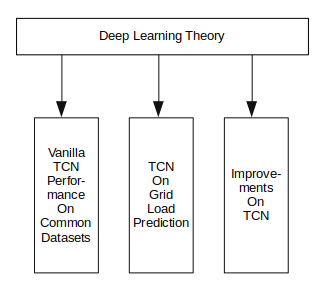
\includegraphics[width=\textwidth]{../Figures/total.png}
    \caption{Total Framework of This Report}
    \label{fig:framework}
\end{figure}
